\section{Teilaufgabe 4}
\begin{aufgabe}
    Zeichnen das asymptotische Bode-Diagramm vom $P_1(s)$ im angehängten 
    leeren Bodediagramm.
\end{aufgabe}
\begin{figure}[h!]
    \centering
    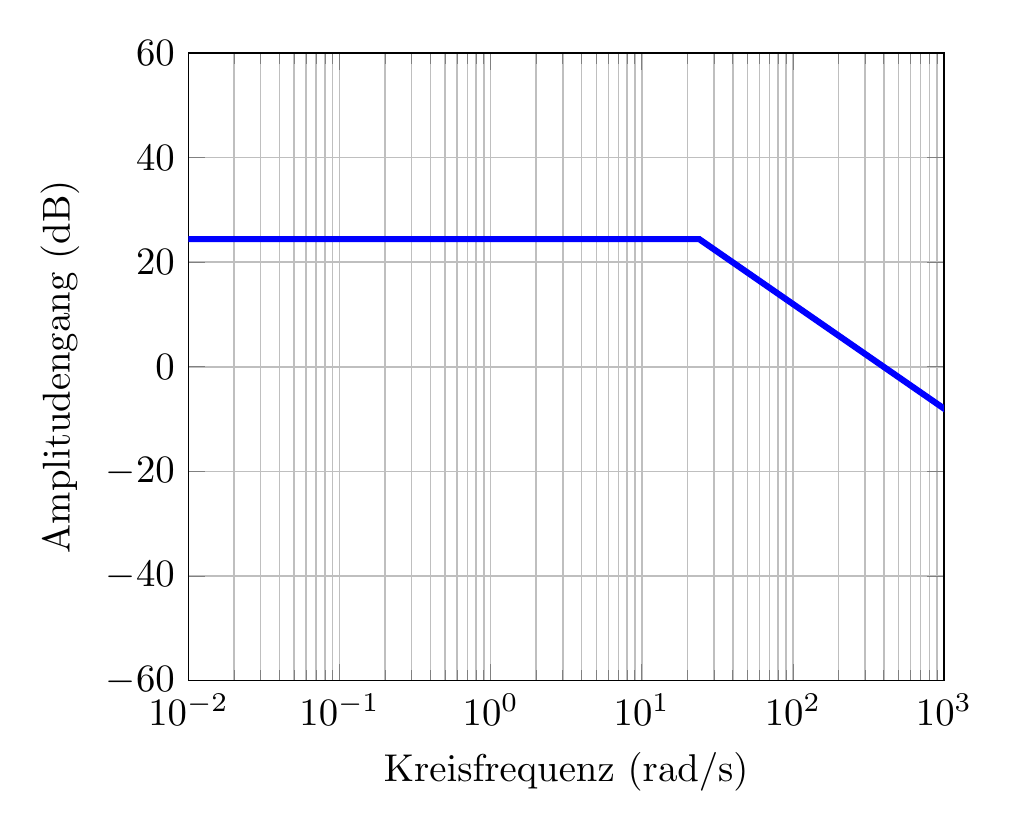
\begin{tikzpicture}[scale=1.4]
        \begin{semilogxaxis}
            [xmin=1e-2, 
                xmax=1e3, 
                ymin=-60, 
                ymax=60, 
                ytick={-60, -40, ..., 60}, 
                xlabel=Kreisfrequenz (rad/s),
                ylabel=Amplitudengang (dB),
                grid=both]
            \addplot[mark=none, color=blue, ultra thick] coordinates 
                {(0.002398,24.430) 
                (23.98,24.430) 
                (2398,-15.57)};
            \node[blue] at (4, 900) {$\omega_e = \frac{1}{\tau} \approx 23.98~s^{-1}$};
            \node[blue] at (-1.5, 750) {$A(0) = K_g \approx 24.43~dB$};
        \end{semilogxaxis}
    \end{tikzpicture}
    \\
    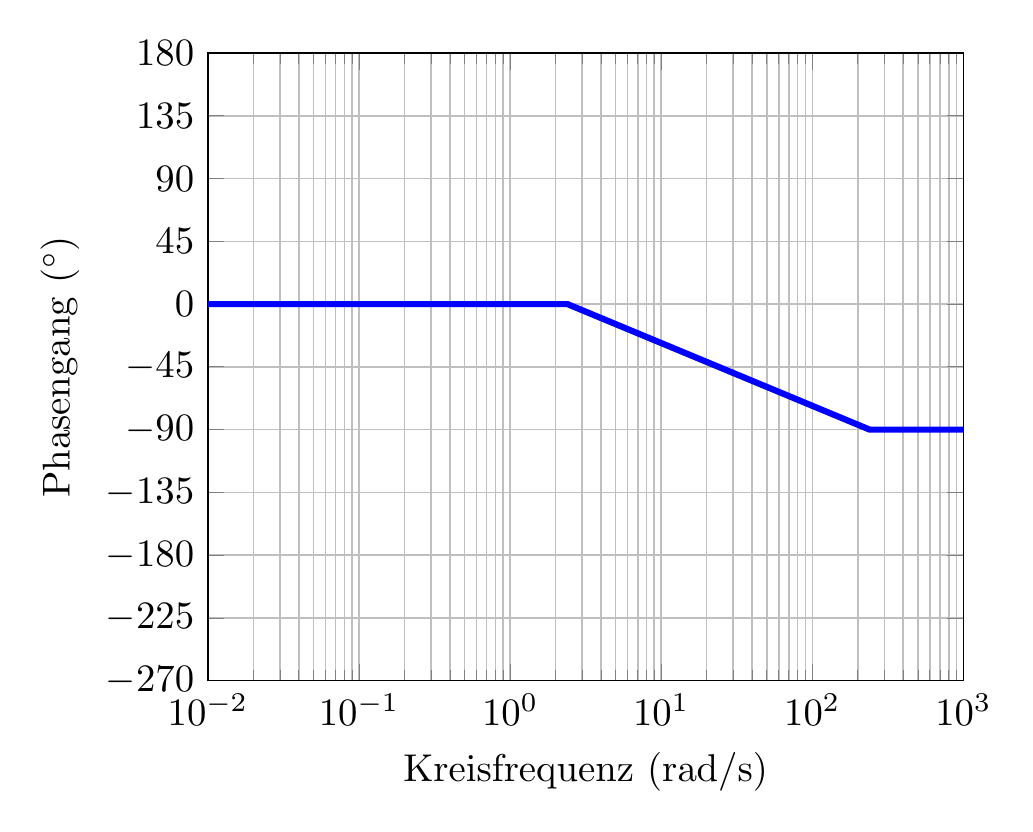
\begin{tikzpicture}[scale=1.4]
        \begin{semilogxaxis}
            [xmin=1e-2, 
                xmax=1e3, 
                ymin=-270, 
                ymax=180, 
                ytick={-270, -225, ..., 180}, 
                xlabel=Kreisfrequenz (rad/s),
                ylabel=Phasengang ($^\circ$),
                grid=both]
            \addplot[mark=none, color=blue, ultra thick] coordinates 
                {(0.002398,0) 
                (2.398,0) 
                (239.8,-90) 
                (2398,-90)};
        \end{semilogxaxis}
    \end{tikzpicture}
\end{figure}
